\section{Data Collection and Preprocessing}
\label{sec:data}

Two complementary benchmark tracks support the evaluation in this paper: a non-executable track scored by text-overlap metrics, and an executable track scored by unit-test execution. Figure~\ref{fig:pipeline_overview} summarizes the overall data pipeline, which proceeds through five stages: raw datasets are collected from multiple sources, schema-normalized to a common format, formatted using instruction templates, deduplicated to remove identical or near-identical examples, and partitioned into train, calibration, and test splits.

\begin{figure}[t]
\centering
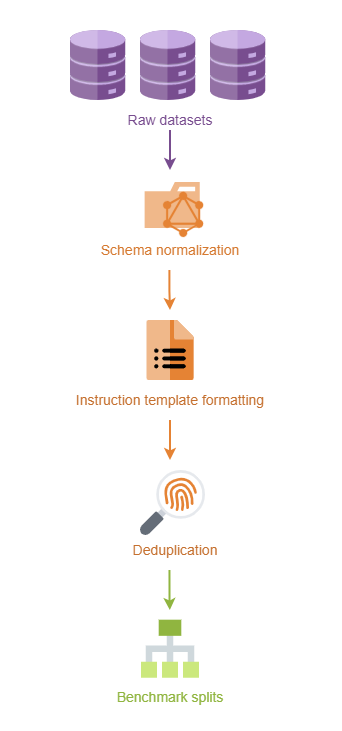
\includegraphics[width=\linewidth]{data_pipeline.png}
\caption{Data collection and preprocessing pipeline. Five sequential stages transform raw datasets from multiple diverse sources into clean, unified benchmark splits for both continual learning evaluation tracks.}
\label{fig:pipeline_overview}
\end{figure}

\subsection{The CodeTask benchmark}
\label{sec:codetask_data}

The CodeTask benchmark is the non-executable track used in this paper. It extends CodeTask-CL \citep{yadav2023exploring}, which combines generation, translation, summarization, and refinement tasks, with four additional tasks to create a longer and more diverse continual learning sequence. The original setting contains four tasks: English-to-Java generation using CONCODE \citep{iyer2018mapping}, Java-to-C\# translation using CodeXGLUE CodeTrans \citep{lu2021codexglue}, Ruby-to-English summarization using CodeSearchNet \citep{husain2019codesearchnet}, and Java-to-Java refinement using BFP \citep{tufano2019empirical}. We add Python generation using KodCode \citep{xu2025kodcode}, Ruby refinement using RunBugRun \citep{prenner2023runbugrun}, C\#-to-English summarization using the-vault-function \citep{nguyen2023vault}, and C++-to-C\# translation using CoST \citep{zhu2022multilingual}. Table~\ref{tab:codetask_stats} lists the eight tasks with their dataset sources and split sizes; Figure~\ref{fig:codetask_sequence} shows the resulting task order.

\begin{table}[t]
\centering
\caption{The CodeTask benchmark used in the non-executable continual learning track.}
\label{tab:codetask_stats}
\scriptsize
\resizebox{\linewidth}{!}{%
\begin{tabular}{llllrrr}
\toprule
Task & Dataset & In & Out & Train & Val. & Test \\
\midrule
Generation & CONCODE & English & Java & 100,000 & 2,000 & 2,000 \\
Translation & CodeXGLUE CodeTrans & Java & C\# & 10,300 & 500 & 1,000 \\
Summarization & CodeSearchNet & Ruby & English & 25,000 & 1,400 & 1,200 \\
Refinement & BFP & Java & Java & 46,600 & 5,800 & 5,800 \\
Generation & KodCode & English & Python & 100,000 & 5,000 & 5,000 \\
Refinement & RunBugRun & Ruby & Ruby & 10,000 & 972 & 1,000 \\
Summarization & the-vault-function & C\# & English & 100,000 & 5,000 & 5,000 \\
Translation & CoST & C++ & C\# & 12,000 & 272 & 410 \\
\bottomrule
\end{tabular}%
}
\end{table}

\begin{figure}[t]
\centering
\resizebox{\linewidth}{!}{%
\begin{tikzpicture}[
  task/.style={rectangle, draw=black!60, rounded corners=3pt,
               minimum width=1.9cm, minimum height=1.15cm,
               text centered, align=center, font=\scriptsize, inner sep=3pt},
  gen/.style={task, fill=blue!13},
  trans/.style={task, fill=orange!15},
  summ/.style={task, fill=green!13},
  ref/.style={task, fill=purple!12},
  arr/.style={-Stealth, thick, draw=black!50}
]
\node[gen]   (t1) {$\mathcal{T}_1$\\Gen\\EN$\to$Java};
\node[trans, right=0.3cm of t1] (t2) {$\mathcal{T}_2$\\Trans\\Java$\to$C\#};
\node[summ,  right=0.3cm of t2] (t3) {$\mathcal{T}_3$\\Summ\\Ruby$\to$EN};
\node[ref,   right=0.3cm of t3] (t4) {$\mathcal{T}_4$\\Ref\\Java$\to$Java};
\node[gen,   right=0.3cm of t4] (t5) {$\mathcal{T}_5$\\Gen\\EN$\to$Python};
\node[ref,   right=0.3cm of t5] (t6) {$\mathcal{T}_6$\\Ref\\Ruby$\to$Ruby};
\node[summ,  right=0.3cm of t6] (t7) {$\mathcal{T}_7$\\Summ\\C\#$\to$EN};
\node[trans, right=0.3cm of t7] (t8) {$\mathcal{T}_8$\\Trans\\C++$\to$C\#};
\draw[arr](t1)--(t2); \draw[arr](t2)--(t3); \draw[arr](t3)--(t4);
\draw[arr](t4)--(t5); \draw[arr](t5)--(t6); \draw[arr](t6)--(t7);
\draw[arr](t7)--(t8);
\end{tikzpicture}}
\caption{The eight-task CodeTask continual learning sequence. Training data from earlier tasks are unavailable once the model advances past each task boundary. Node color indicates task type: blue for generation, orange for translation, green for summarization, purple for refinement.}
\label{fig:codetask_sequence}
\end{figure}

The additional tasks widen the range of languages and task types and introduce stronger distribution shifts: some tasks map natural language to code, some map code to code, and some map code to natural language. This mix makes the sequence more representative of real code-assistant workloads and better suited to studying when knowledge should transfer between tasks and when it should remain separated; restricting the sequence to one type of generation problem would risk conflating narrow adaptation with genuine continual learning ability.

Each dataset is cast into a unified instruction-style sequence-to-sequence format, since the source datasets use different schemas (natural-language intent and code snippet; buggy and repaired code; source code and docstring). To avoid the model relying on a single memorized prompt format, each example is wrapped with a template drawn from a pool of $N=20$ training templates per task type; at test time the pool expands to $M=30$ templates, so the test-time instructions include both familiar and unseen phrasing.

\subsection{The executable benchmark and deduplication pipeline}
\label{sec:exec_data}

The executable benchmark evaluates multilingual code generation under execution-based grading. Training data are drawn from OSS-Instruct \citep{wei2023magicoder} and McEval-Instruct \citep{chai2024mceval}; test data are drawn from McEval \citep{chai2024mceval}. All subsets cover the same nine programming languages: Python, C++, C\#, Java, Rust, Swift, PHP, TypeScript, and Shell. Unlike the CodeTask benchmark, each test example provides a problem description together with unit tests rather than a single reference output, and success is defined by whether the generated program passes the tests rather than by textual similarity to a reference solution, following the execution-based evaluation methodology of \citet{chen2021evaluating}.

Table~\ref{tab:exec_stats} summarizes the train, calibration, and test splits. OSS-Instruct is the largest training source (41,613 examples); McEval-Instruct adds 8,985 more balanced examples; McEval serves as the held-out test set. The calibration split --- used for candidate generation and for fitting the traceback router described in Section~\ref{sec:methodology} --- is assembled from the sanitized MBPP test split for Python \citep{austin2021program} and from the \texttt{mbpp-\textit{ext}} configuration of MultiPL-E for the remaining eight languages \citep{cassano2023multipl}; MultiPL-E does not provide reference solutions for these languages, so only pass/fail execution feedback is available for them. All calibration and test data are standardized to match the McEval instruction and test format.

\begin{table}[t]
\centering
\caption{Statistics of the executable benchmark subsets.}
\label{tab:exec_stats}
\scriptsize
\resizebox{\linewidth}{!}{%
\begin{tabular}{lrrrrrrrrrr}
\toprule
Split & Py & C++ & C\# & Java & Rust & Swift & PHP & TS & Shell & Total \\
\midrule
Train & 5,699 & 5,697 & 5,449 & 5,565 & 5,692 & 5,496 & 5,576 & 5,698 & 5,726 & 50,598 \\
Calib. & 426 & 397 & 386 & 386 & 354 & 396 & 397 & 390 & 382 & 3,514 \\
Test & 50 & 50 & 50 & 53 & 53 & 50 & 50 & 50 & 50 & 456 \\
\bottomrule
\end{tabular}%
}
\end{table}

The benchmark also brings multilingual adaptation into the continual learning setting: the same code-generation task repeats across nine languages that differ in syntax, standard libraries, and idiomatic patterns, so a continual learner may experience both positive transfer and interference across languages that the CodeTask benchmark, with its diversity of task types, does not directly test. Compared with CodeTask, the executable benchmark is narrower in task type but stronger in functional evaluation, isolating a single question: can the model keep learning to generate working programs across languages over time?

Because the executable benchmark is graded by execution, an undetected overlap between training and test examples would inflate reported scores by rewarding memorization rather than generalization, an effect that matters even more for a continual learner, whose apparent retention could otherwise reflect data leakage rather than genuine forward or backward transfer. The construction of the executable benchmark therefore includes a two-stage deduplication pipeline, illustrated in Figure~\ref{fig:near_dedup}.

\textbf{Exact deduplication.} Instruction text is whitespace-normalized and hashed with SHA-256 \citep{nist2015securehash}; examples sharing a hash are grouped into a cluster and reduced to one canonical representative. This stage removes verbatim copies but not near-identical problems that differ only by renamed identifiers or reworded descriptions.

\textbf{Near deduplication.} A stronger normalization is applied first --- Unicode normalization, prose/code separation, placeholder abstraction, identifier generalization to generic tokens, and import/punctuation normalization --- after which each example is represented as a set of token $n$-gram shingles. Comparing all shingle-set pairs directly is $O(N^2)$ and infeasible at scale, so MinHash is used to approximate Jaccard similarity efficiently: given $m$ independent hash functions, the signature of a shingle set $S$ is $\mathrm{MH}(S)=(\min_{s\in S}h_1(s),\ldots,\min_{s\in S}h_m(s))$, with the property $\Pr[\min h(S_A)=\min h(S_B)]=J(S_A,S_B)$ \citep{broder1997resemblance}. Locality-Sensitive Hashing (LSH) then restricts pairwise comparison to signatures sharing a band \citep{indyk1998approximate}, and each surviving candidate pair is scored with the exact Jaccard similarity $J(S_A,S_B)=|S_A\cap S_B|/|S_A\cup S_B|$ \citep{jaccard1901distribution}; a pair with $J\geq\theta$ is recorded as a near duplicate.

\begin{figure}[t]
\centering
\resizebox{\linewidth}{!}{%
\begin{tikzpicture}[
  node distance=0.5cm,
  box/.style={rectangle, draw=black!65, rounded corners=3pt,
              minimum width=5.0cm, minimum height=0.72cm,
              text centered, font=\small, inner sep=4pt},
  procbox/.style={box, fill=orange!13},
  decbox/.style={box, fill=red!9},
  outbox/.style={box, fill=green!12},
  arr/.style={-Stealth, thick, draw=black!60},
]
\node[procbox] (norm) {Stronger Text Normalization};
\node[procbox, below=0.5cm of norm] (shin) {Shingling (token $n$-grams)};
\node[procbox, below=0.5cm of shin] (mh)   {MinHash Signatures};
\node[procbox, below=0.5cm of mh]   (lsh)  {LSH Candidate Retrieval};
\node[procbox, below=0.5cm of lsh]  (jac)  {Exact Jaccard Scoring};
\node[decbox,  below=0.5cm of jac]  (thr)  {Threshold Filter ($J \geq \theta$)};
\node[outbox,  below=0.5cm of thr]  (dup)  {Near-Duplicate Pairs};
\draw[arr](norm)--(shin); \draw[arr](shin)--(mh);
\draw[arr](mh)--(lsh);   \draw[arr](lsh)--(jac);
\draw[arr](jac)--(thr);  \draw[arr](thr)--(dup);
\end{tikzpicture}}
\caption{Near-deduplication pipeline. Normalization and shingling produce set representations; MinHash enables approximate similarity estimation; LSH restricts the search space to candidate pairs; exact Jaccard scoring provides the final decision.}
\label{fig:near_dedup}
\end{figure}

Exact-duplicate clusters are filtered and near-duplicate pairs that cross the train--test boundary are removed; this train--test filtering step is the primary safeguard against the model solving a test problem because it has seen an almost-identical version during training rather than because it generalized. The final stage standardizes all processed outputs into a common schema across splits, with shared fields index, language, instruction, solution, and test, so deduplication is integrated into the main benchmark construction pipeline rather than a separate post-hoc cleanup step.
